% figures/ai-build-buy.tex
% Standalone TikZ: AI Build vs. Buy vs. API 2x2 matrix (ch.17 data-and-ai-strategy).
% Axes: horizontal = task specificity (generic -> proprietary);
%        vertical   = proprietary data advantage (low -> high).
% Compiled to figures/ai-build-buy.pdf via tools/build-figures.sh.
\documentclass[tikz,border=4pt]{standalone}
\usepackage{tikz}
\usetikzlibrary{arrows.meta,positioning}

\definecolor{vcblue}{HTML}{1A5276}
\definecolor{vcteal}{HTML}{0E6655}
\definecolor{vcgray}{HTML}{4D4D4D}

\begin{document}
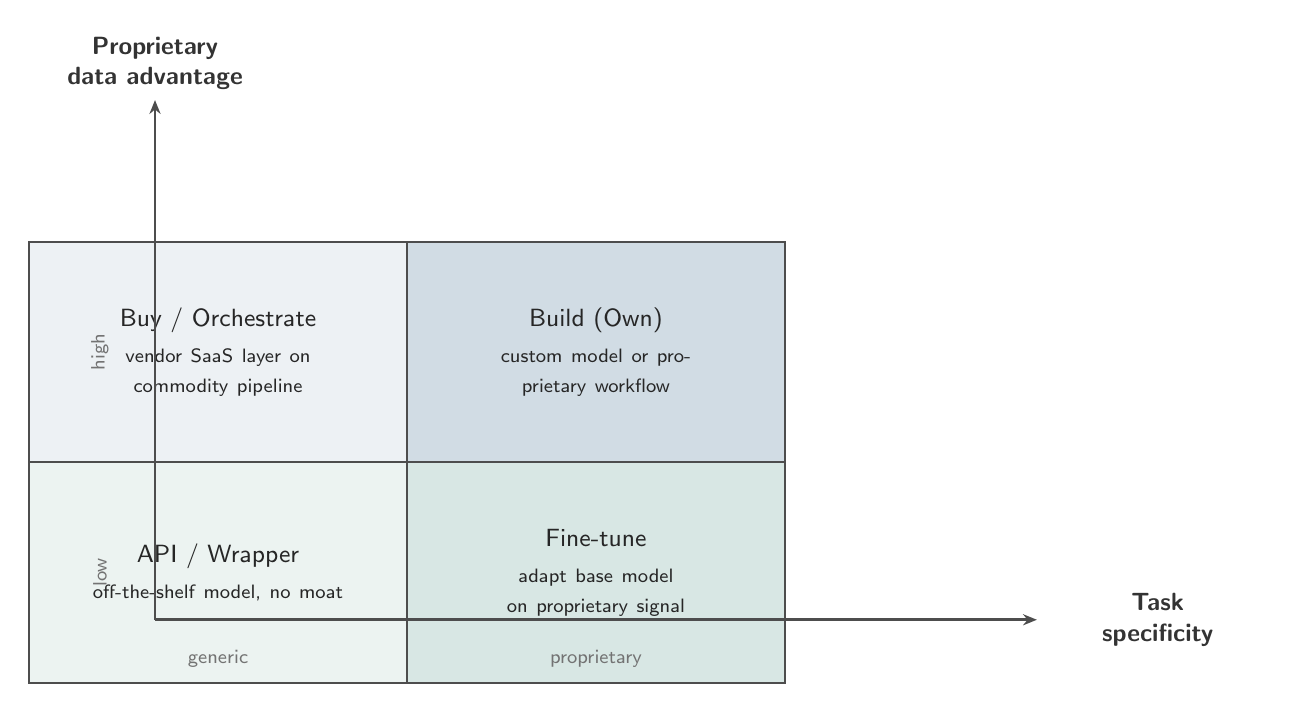
\begin{tikzpicture}[
  cell/.style={draw=vcgray, line width=0.7pt, align=center, text width=40mm,
               minimum width=48mm, minimum height=28mm, font=\sffamily\small, text=black!85},
  axislbl/.style={font=\sffamily\small\bfseries, text=black!80, align=center},
  sublbl/.style={font=\sffamily\scriptsize, text=black!55, align=center},
  arr/.style={-{Stealth[length=5pt,width=4pt]}, vcgray, line width=1pt},
]

% Quadrant cells (SW, SE, NW, NE). Sub-text wraps via text width (no nested line breaks).
\node[cell, fill=vcteal!8]  (sw) at (0,0)      {API / Wrapper\\[2pt]{\scriptsize off-the-shelf model, no moat}};
\node[cell, fill=vcteal!16] (se) at (48mm,0)   {Fine-tune\\[2pt]{\scriptsize adapt base model on proprietary signal}};
\node[cell, fill=vcblue!8]  (nw) at (0,28mm)   {Buy / Orchestrate\\[2pt]{\scriptsize vendor SaaS layer on commodity pipeline}};
\node[cell, fill=vcblue!20] (ne) at (48mm,28mm){Build (Own)\\[2pt]{\scriptsize custom model or proprietary workflow}};

% Axis arrows
\draw[arr] (-8mm,-6mm) -- (-8mm,60mm)
  node[axislbl, above, text width=30mm] {Proprietary\\data advantage};
\draw[arr] (-8mm,-6mm) -- (104mm,-6mm)
  node[axislbl, right, text width=28mm] {Task\\specificity};

% Axis tick labels
\node[sublbl] at (0,-11mm)   {generic};
\node[sublbl] at (48mm,-11mm){proprietary};
\node[sublbl, rotate=90] at (-15mm,0)    {low};
\node[sublbl, rotate=90] at (-15mm,28mm) {high};

\end{tikzpicture}
\end{document}
